\section{Theory}\label{sec:theory}

This section discusses the theory behind the models used in the 

\subsection{Linear regression}

The regression model will be for the sake of convenience be expressed as the following expression
$$
\left(\vec{F}\circ \mathbf{A}\right)\vec{\beta}=\vec{y}+\vec{\varepsilon}
$$

Where $\vec{F}$ is a vector function with following domain $\vec{F}:\mathbb{R}^{m\times n}\to \mathbb{R}^{m\times p}$ where $m,p\in \mathbb{N}$, $\mathbf{A}$ is the data in matrix form with dimensions $\mathbb{R}^{m\times n}$, $\vec{\beta}$ is the regression terms, $\vec{y}$ is the target (TJM), and $\vec{\varepsilon}$ is the error from modelling. The $\circ$ operator is the composition of $\vec{F}$ and $\mathbf{A}$, is a short way of writing $\vec{F}(\mathbf{A})$.

\subsection[Plauborg Regression]{Plauborg linear regression model with Fourier terms}

Making a linear regression model for soil temperature sensitive to time without introducing more computational heavy operation would be to introduce features that reflect time. In the paper \citetitle{plauborg_simple_2002} the author chose to extend the features from air temperature to include also day of year and the air temperature from those days. This means the following F function that \citeauthor{plauborg_simple_2002} used would be 
$$
\vec{F} := [air_t \; air_{t-1}\; air_{t-2}\; air_{t-3}\; \sin(\omega t) \; \cos(\omega t)\; \sin(2*\omega t)\; \cos(2*\omega t)]^T
$$

Where $air_t$ is the air temperature at time $t$ expressed in day of year, $\omega$ is the angular frequency to make the argument of sine and cosine expressed in radians. The sine/cosine elements in the F function represent the variations through the day by fitting $\vec{\beta}$ to the yearly variation. To adapt the authors model to an hourly time unit would be to either
\begin{enumerate}
	\item Extend the F function to include a larger $\omega$ coefficient to reflect hourly oscillations in conjunction with daily fluxiations
	\item Refit the Fourier terms with a larger $\omega$ coefficient to make the oscillations more representative of daily temperature changes.
\end{enumerate}

The larger coefficient could be expressed as $2\pi/24$ while the smaller $\omega$ for daily values would be rescaled to $2\pi/8760$.

\subsection[Rankin algorithm]{Rankin's Forward-Euler method of simplified heat flow in snow cowered soil}\cite{rankinen_simple_2004}


\subsection{Long Short Term Memory model}

\begin{figure}[ht]
	\centering
	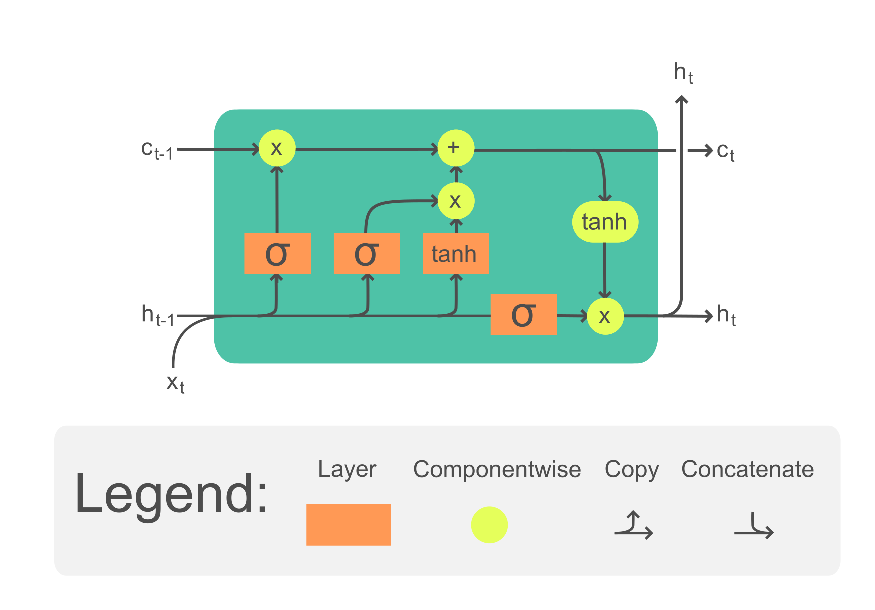
\includegraphics[width=0.7\linewidth]{figures/LSTM_Cell}
	\caption{LSTM cell  Artist: \textcite{chevalier_english_2018}}
	\label{fig:lstmcell}
\end{figure}

\subsection[ILSTM]{Attention aware LSTM model}

